
%-------------------------------------------------------------------
\chapter{\textbf{SCATMA Basics and Requirements}}
\label{ch:basics}
% \chaptermark{Fourier Transform Theory}
%-------------------------------------------------------------------

This chapter presents the instant water heating problem, the SCATMA solution and the main concerns in selecting an energy storage medium for this application. 

\section{Heating Still and Flowing Water}
% \sectionmark{Continuous-Time Representation}

The amount of energy $E$ [in J] required to raise the temperature of $l$ litres of water inside a perfectly insulated container by $\Delta\theta$~[$\deg$C] is 
%
\begin{equation}
\label{eq:stil_energy}
  E\eq\rho lC\Delta\theta
\end{equation}
%
where $\rho$ is the density of water [kg\,L$^{-1}$], $C$ is the specific heat capacity of water~[J\,kg$^{-1}$\,$\deg$C$^{-1}$].
If the temperature rise $\Delta\theta$ is to occur within time $\Delta T$, the required average heating power $P$ can be calculated as
%
\begin{equation}
\label{eq:still_power}
    P\eq\frac{E}{\Delta T}\eq\frac{\rho lC\Delta\theta}{\Delta t} 
\end{equation}
%
where no losses are assumed at the source or in the power transfer path.
Inserting Eq.(\ref{eq:stil_energy}) gives
%
\begin{equation}
\label{eq:still_power_rearrange}
P\eq\frac{l}{\Delta t}\rho C\Delta\theta\eq Q\rho C\Delta\theta
\end{equation}
%
where $Q$ is the water flow rate [Lmin$^{-1}$]. This equation describes heating a flow of water with~$100\%$ heat transfer efficiency at the heating element surface.
%




%-------------------------------------------------------------------
\subsection{Electric Kettle Example}

Take the static example of a 230~V, 2.3~kW rated 4-litre electric kettle. It takes 9.7 min to raise the temperature of 4~L of water from 20$\deg$C room temperature to 100$\deg$C. This result follows form Eq.~(\ref{eq:still_power}),
%
\begin{equation}
\label{eq:kettle _still}
2300~\text{W} \eq \frac{(1~\text{kg\,L}^{-1})(4200~\text{J\,kg}^{-1}\,\deg \text{C}^{-1}) (80\deg \text{C}}{\Delta t})~~~ \implies~~~ \Delta t \eq 9.74~ \text{min}
\end{equation}



If the same power input is applied to water flowing inside a perfectly insulated tube, then the maximum permissible flow rate for the same temperature rise is $0.41$~L\,min$^{-1}$,
%
\begin{equation}
\label{eq:kettle _flow}
2300~\text{W}\eq\left(\frac{4~\text{L}}{9.74~\text{min}}\right)\rho C\,(80\deg \text{C})~~~\implies ~~~ Q\,\eq\,0.41~\text{L\,min}^{-1}
\end{equation}


Similarly if the temperature rise is halved to 40$\deg$C then the maximum flow rate for the same heater power would be doubled to 0.81~L\,min$^{-1}$. If the flow rate needs to be increased ten-fold to 8~Lmin$^{-1}$ for the same 40$\deg$C temperature rise, then a ten-fold higher power source of 23~kW is required. 

\begin{figure}[t]
	\centering
	 \resizebox{16cm}{!}{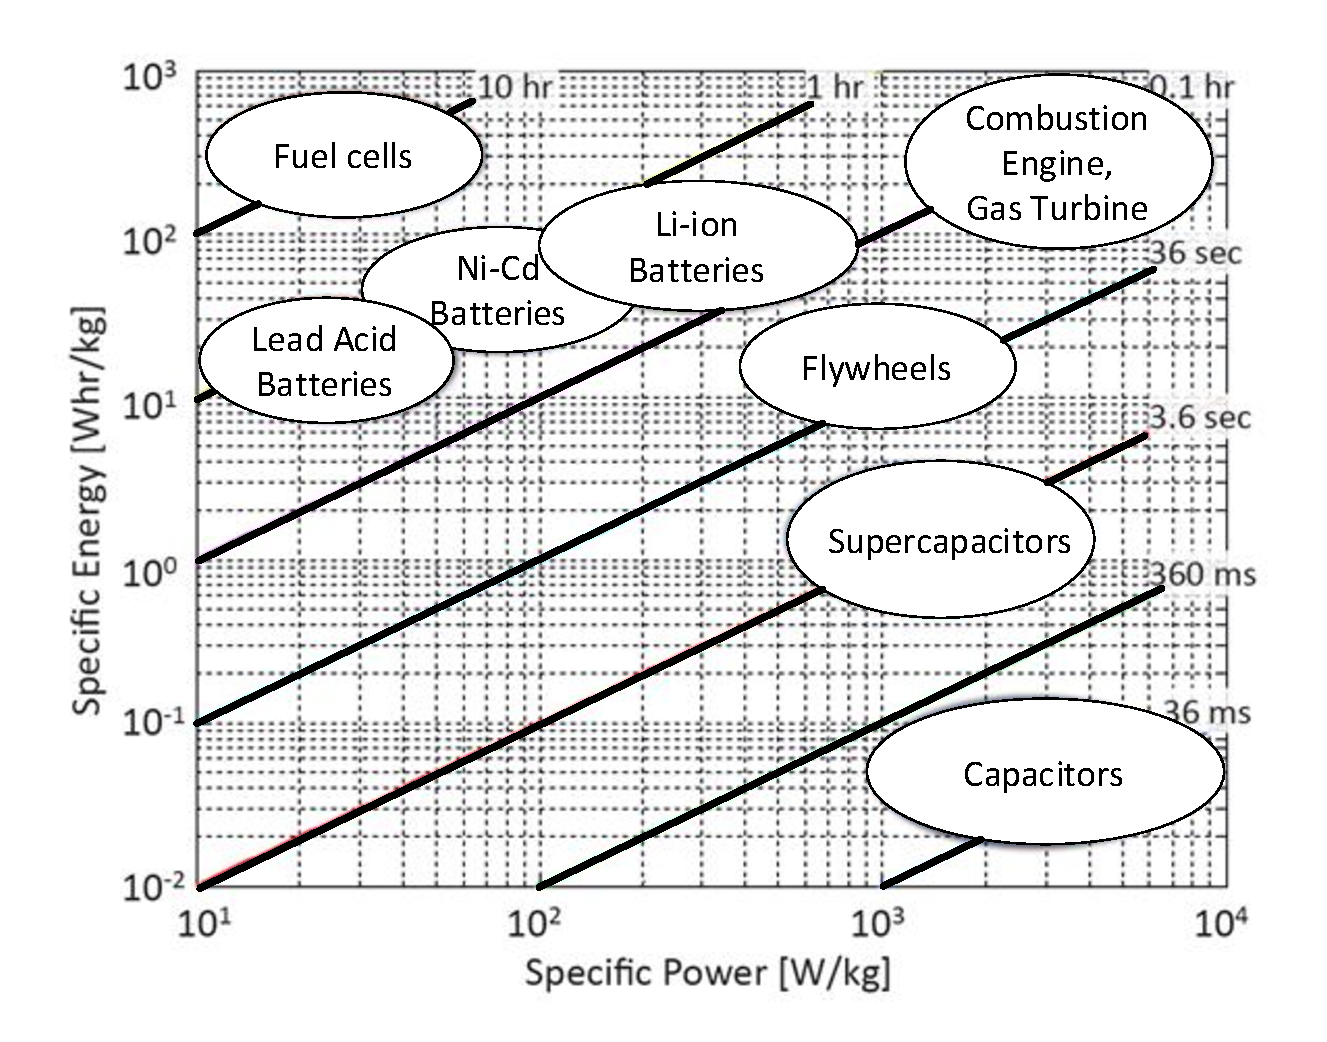
\includegraphics[draft=false]{_figs/th_ragone_vco}}
	%\includegraphics[draft=false]{_figs/Ragone_plot}
	\caption[ Ragone plot]
		{%
		\label{fg:Ragone_plot}
		\centering
		Ragone plot of various energy storage/propulsion devices and their ``charge" times.  Adapted from US Defense Logistics Agency Report~\cite{Obey:09} 
	}
\end{figure}

